\chapter{Features and Primitives}

\section{Image Processing}

\subsection{Linear Filtering}

\subsection{Non-linear filters and other neighborhood operators}

An example of this is the \textbf{Median Filter}, which substitutes each pixel value with the \textit{median} of the distribution of the neighborhood. Since the median is robust to outliers, median filtering helps in filtering out the \textbf{shot noise}, where linear filters, like Gaussian smoothing perform poorly. It is robust to outliers.

\begin{figure}[h]
    \centering
    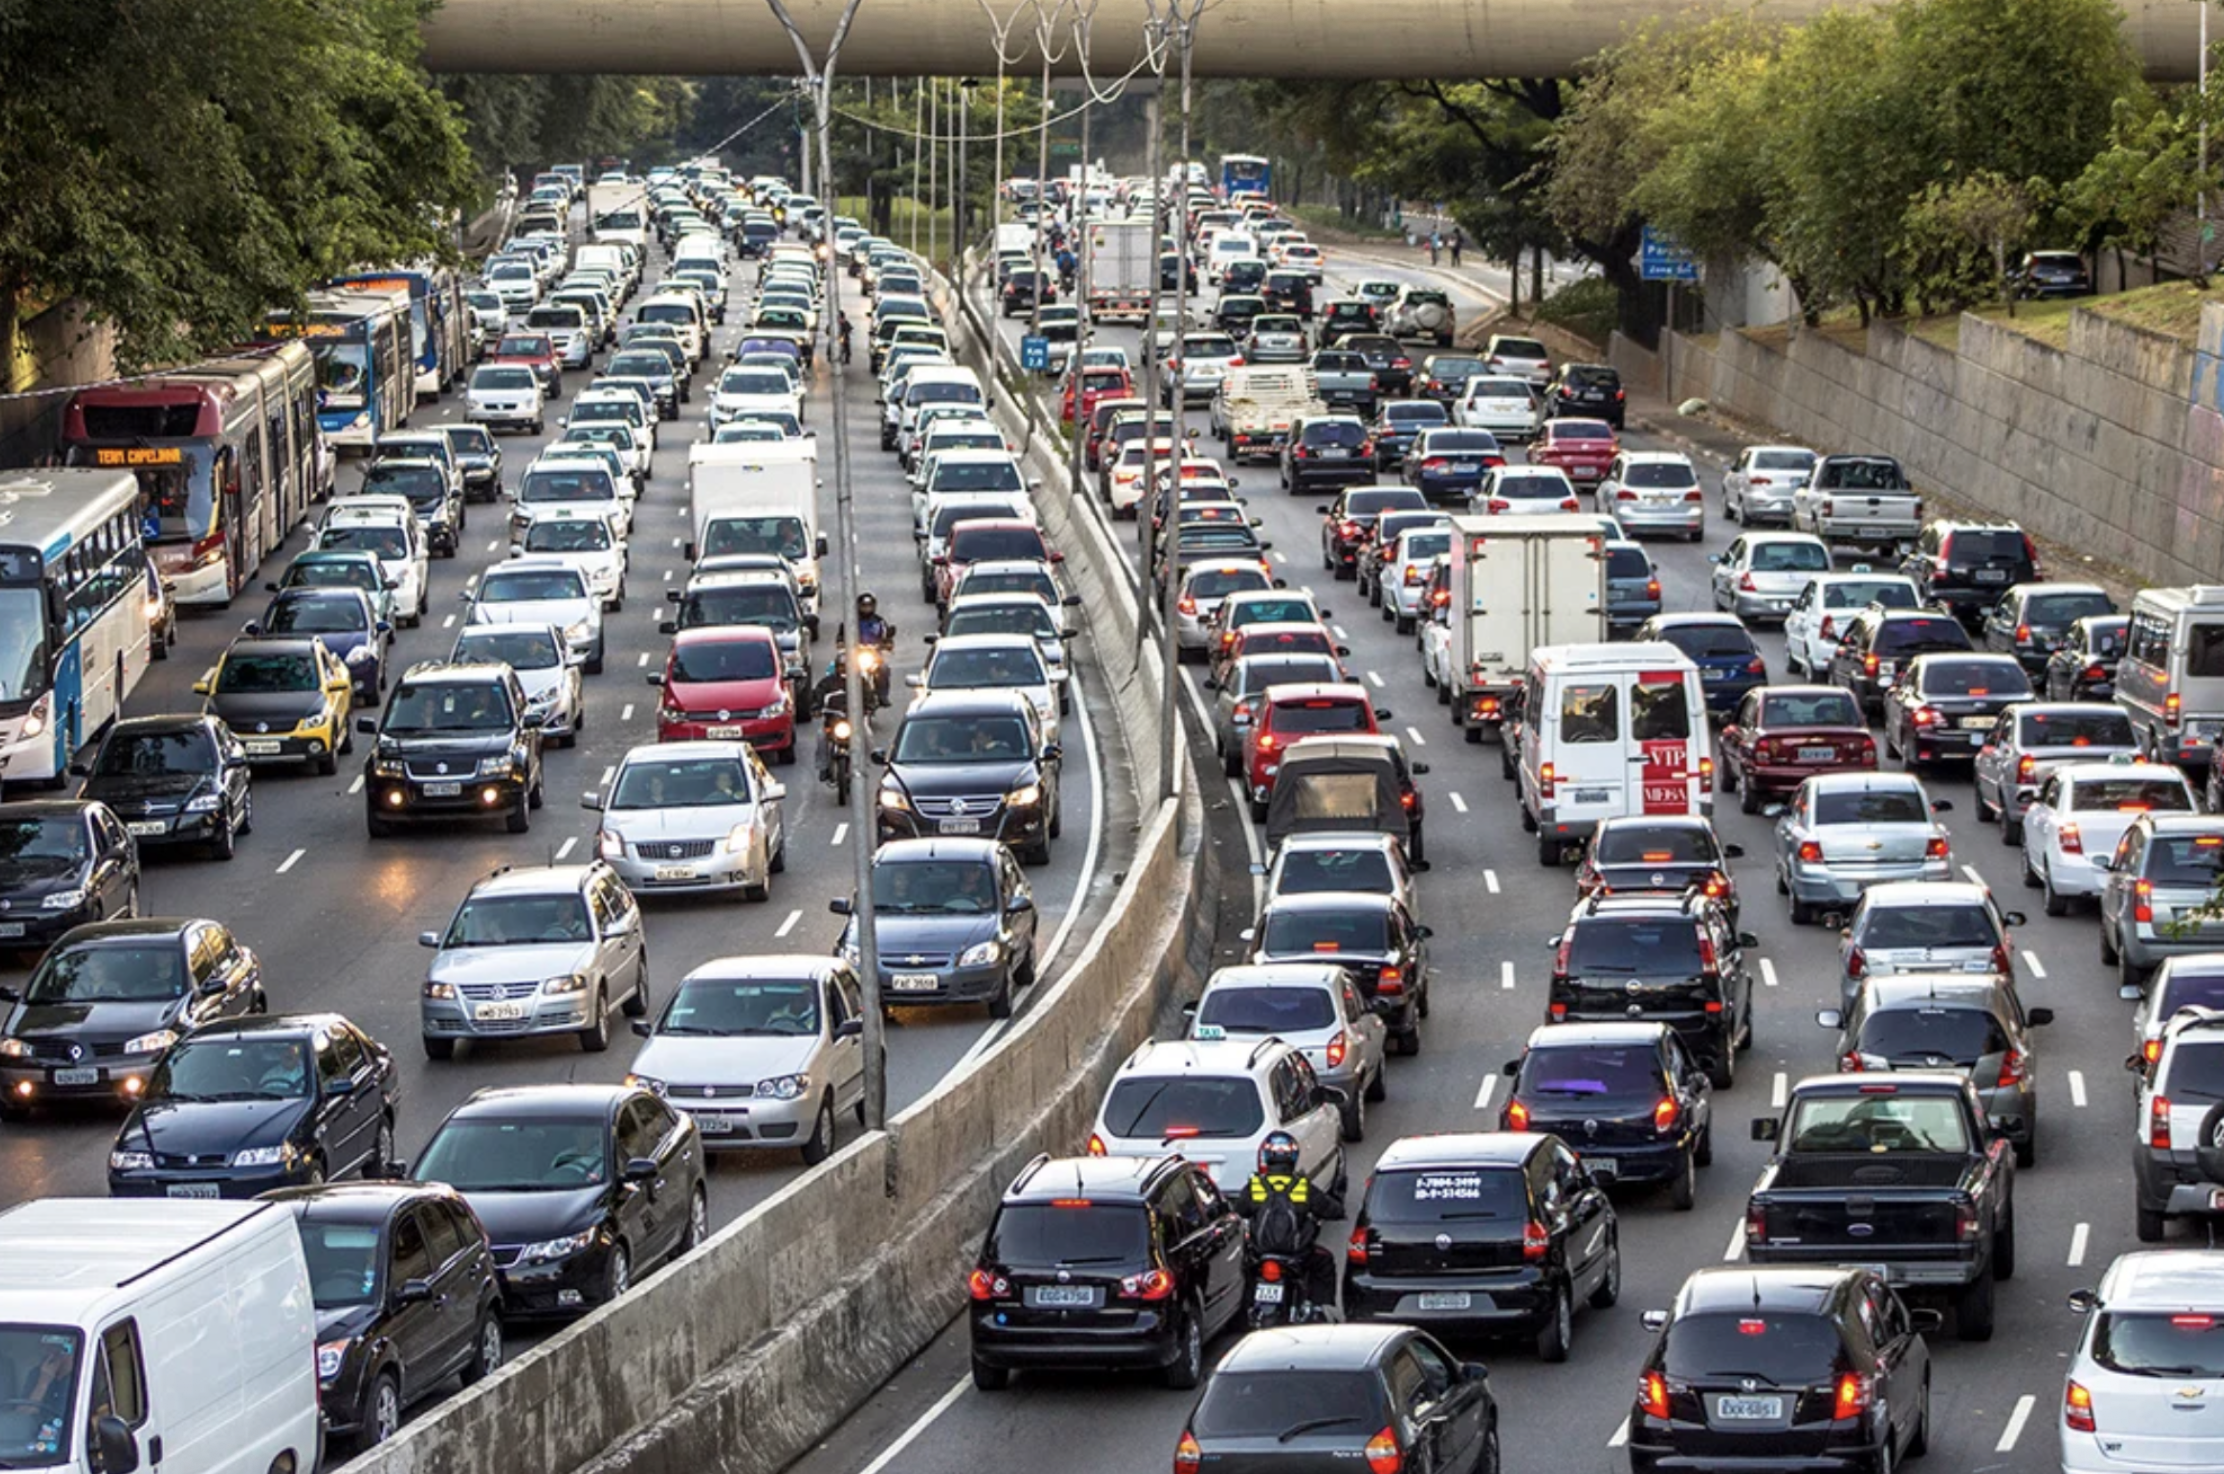
\includegraphics[width=\textwidth]{assets/ch3/1.png}
    \caption{}
    \label{fig:median_filter}
\end{figure}

We can go on using different versions of the median filter, considering also mean filters:
\begin{itemize}
    \item \textbf{$\alpha$-trimmed mean filter}: it is a non-linear filter that averages together all the pixels except for the $\alpha$ fraction that are the smallest and the largest;
    \item \textbf{Weighted median filter}: corresponds to the median of a weighted distribution, where each pixel appears a number of times depending on its distance from the center of the neighborhood. It can be show to be equivalent to the following optimization problem:
    \begin{align}
        \min_{g(i,j)}\sum_{k,k} w(k,l) |f(i+k,j+l) - g(i,j)|^p 
    \end{align}
    where $-W \leq k,l \leq W$ and $p=1$. For $p=2$ we have the weighted mean filter.
\end{itemize}



\subsection{Image warping}

\subsection{Multi-resolution representations}

